\documentclass[12pt]{standalone}
\usepackage[utf8]{inputenc}
\usepackage[T1]{fontenc}
\usepackage{times}
\usepackage{amsmath,amssymb}
\usepackage[dvipsnames,svgnames]{xcolor}
\usepackage{tikz}
\usetikzlibrary{decorations.pathreplacing, calc, positioning, shapes.geometric, shapes.symbols, arrows.meta, backgrounds, fit, shapes.misc}
\definecolor{RED}{rgb}{1,0,0}
\definecolor{dmrsfill}{HTML}{CDE2FB}
\definecolor{winblue}{HTML}{0D366B}
\definecolor{inksec}{HTML}{52514E}
\begin{document}
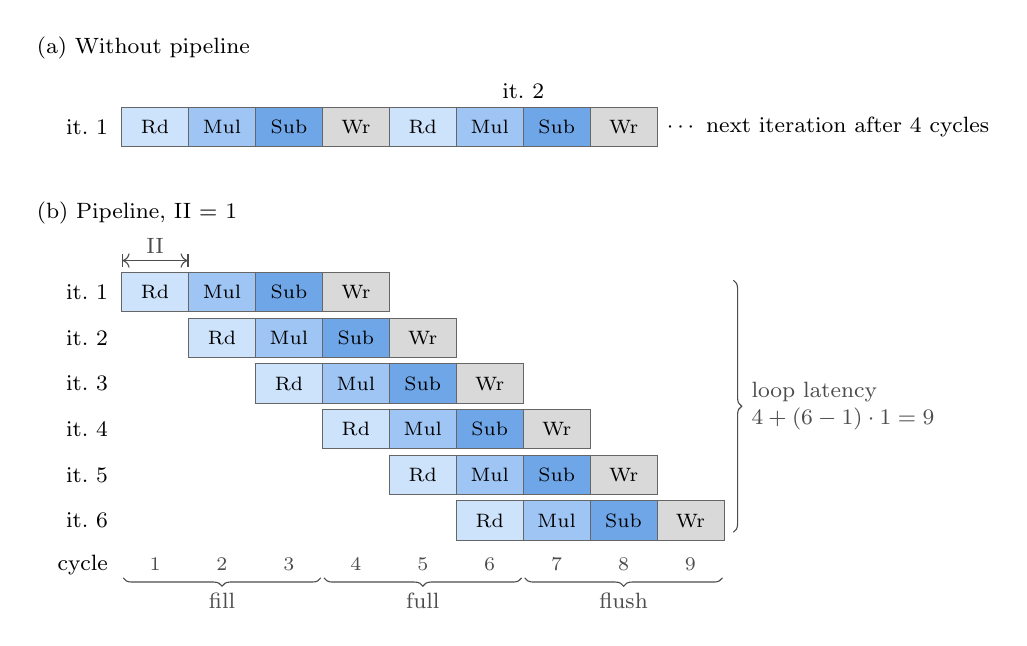
\begin{tikzpicture}[font=\fontsize{8.5}{10}\selectfont,
  est/.style={draw=black!60, fill=#1, minimum width=0.85cm, minimum height=0.50cm, inner sep=0pt, line width=0.3pt},
  est/.default=white]
\def\u{0.85}\def\h{0.58}
\definecolor{e1}{HTML}{CDE2FB}\definecolor{e2}{HTML}{9EC5F4}\definecolor{e3}{HTML}{6FA6E8}\definecolor{e4}{HTML}{D9D9D9}
% estágios de uma iteração: Rd, Mul, Sub, Wr (latência de 4 ciclos)
\newcommand{\iter}[3]{% #1 = ciclo de início (0-index), #2 = linha, #3 = rótulo
  \node[est=e1] at (#1*\u+0.5*\u, -#2*\h) {\fontsize{7}{8}\selectfont Rd};
  \node[est=e2] at (#1*\u+1.5*\u, -#2*\h) {\fontsize{7}{8}\selectfont Mul};
  \node[est=e3] at (#1*\u+2.5*\u, -#2*\h) {\fontsize{7}{8}\selectfont Sub};
  \node[est=e4] at (#1*\u+3.5*\u, -#2*\h) {\fontsize{7}{8}\selectfont Wr};
  \node[left] at (-0.05, -#2*\h) {#3};}
% (a) sem pipeline
\node[anchor=west] at (-1.2, 1.00) {(a) Without pipeline};
\iter{0}{0}{it.~1}
\begin{scope}[shift={(4*\u,0)}]
  \node[est=e1] at (0.5*\u,0) {\fontsize{7}{8}\selectfont Rd};
  \node[est=e2] at (1.5*\u,0) {\fontsize{7}{8}\selectfont Mul};
  \node[est=e3] at (2.5*\u,0) {\fontsize{7}{8}\selectfont Sub};
  \node[est=e4] at (3.5*\u,0) {\fontsize{7}{8}\selectfont Wr};
\end{scope}
\node at (6*\u, 0.45) {it.~2};
\node[right] at (8*\u, 0) {$\cdots$ next iteration after 4 cycles};
% (b) com pipeline, II = 1, 6 iterações
\begin{scope}[shift={(0,-2.10)}]
\node[anchor=west] at (-1.2, 1.00) {(b) Pipeline, II = 1};
\foreach \i in {0,...,5} { \pgfmathtruncatemacro{\r}{\i+1} \iter{\i}{\i}{it.~\r} }
% eixo dos ciclos
\foreach \c in {1,...,9} \node[text=black!70] at (\c*\u-0.5*\u, -6*\h+0.02) {\fontsize{7}{8}\selectfont\c};
\node[left] at (-0.05, -6*\h+0.02) {cycle};
% II
\draw[black!70, |<->|, line width=0.4pt] (0,0.40) -- (\u,0.40) node[midway, above=-1pt] {II};
% enchimento, regime e esvaziamento
\draw[decorate, decoration={brace, mirror, amplitude=3pt}, black!70, line width=0.4pt] (0.02,-6*\h-0.15) -- (3*\u-0.02,-6*\h-0.15) node[midway, below=2pt, align=center] {fill};
\draw[decorate, decoration={brace, mirror, amplitude=3pt}, black!70, line width=0.4pt] (3*\u+0.02,-6*\h-0.15) -- (6*\u-0.02,-6*\h-0.15) node[midway, below=2pt, align=center] {full};
\draw[decorate, decoration={brace, mirror, amplitude=3pt}, black!70, line width=0.4pt] (6*\u+0.02,-6*\h-0.15) -- (9*\u-0.02,-6*\h-0.15) node[midway, below=2pt, align=center] {flush};
\draw[decorate, decoration={brace, amplitude=3pt}, black!70, line width=0.4pt] (9*\u+0.12,0.15) -- (9*\u+0.12,-5*\h-0.15) node[midway, right=3pt, align=left] {loop latency\\$4 + (6-1)\cdot 1 = 9$};
\end{scope}
\end{tikzpicture}
\end{document}
